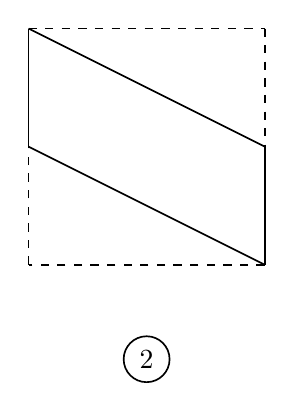
\begin{tikzpicture}[x=1cm,y=1cm,font=\normalsize,
 geometry edge/.style={solid,line width=.6pt},
 geometry mark/.style={solid,line width=.6pt},
 geometry label/.style={font=\normalsize,inner sep=2pt}]
\coordinate (Q1) at (0,3);
\coordinate (Q2) at (3,3);
\coordinate (Q3) at (3,0);
\coordinate (Q4) at (0,0);
\coordinate (L2) at (0,1.5);
\coordinate (R1) at (3,1.5);
\coordinate (NC) at (1.5,-1.2);
\draw[geometry edge,dashed] (Q1)--(Q2);
\draw[geometry edge,dashed] (Q2)--(Q3);
\draw[geometry edge,dashed] (Q3)--(Q4);
\draw[geometry edge,dashed] (Q4)--(Q1);
\draw[geometry edge] (Q1)--(L2);
\draw[geometry edge] (Q1)--(R1);
\draw[geometry edge] (L2)--(Q3);
\draw[geometry edge] (R1)--(Q3);
\node[draw,circle,inner sep=3pt,line width=.6pt] at (NC) {2};
\end{tikzpicture}